\chapter{Diseño e implementación} % Main chapter title

\label{Chapter3} % Change X to a consecutive number; for referencing this chapter elsewhere, use \ref{ChapterX}

\definecolor{mygreen}{rgb}{0,0.6,0}
\definecolor{mygray}{rgb}{0.5,0.5,0.5}
\definecolor{mymauve}{rgb}{0.58,0,0.82}

%%%%%%%%%%%%%%%%%%%%%%%%%%%%%%%%%%%%%%%%%%%%%%%%%%%%%%%%%%%%%%%%%%%%%%%%%%%%%
% parámetros para configurar el formato del código en los entornos lstlisting
%%%%%%%%%%%%%%%%%%%%%%%%%%%%%%%%%%%%%%%%%%%%%%%%%%%%%%%%%%%%%%%%%%%%%%%%%%%%%
\lstset{ %
  backgroundcolor=\color{white},   % choose the background color; you must add \usepackage{color} or \usepackage{xcolor}
  basicstyle=\footnotesize,        % the size of the fonts that are used for the code
  breakatwhitespace=false,         % sets if automatic breaks should only happen at whitespace
  breaklines=true,                 % sets automatic line breaking
  captionpos=b,                    % sets the caption-position to bottom
  commentstyle=\color{mygreen},    % comment style
  deletekeywords={...},            % if you want to delete keywords from the given language
  %escapeinside={\%*}{*)},          % if you want to add LaTeX within your code
  %extendedchars=true,              % lets you use non-ASCII characters; for 8-bits encodings only, does not work with UTF-8
  %frame=single,	                % adds a frame around the code
  keepspaces=true,                 % keeps spaces in text, useful for keeping indentation of code (possibly needs columns=flexible)
  keywordstyle=\color{blue},       % keyword style
  language=[ANSI]C,                % the language of the code
  %otherkeywords={*,...},           % if you want to add more keywords to the set
  numbers=left,                    % where to put the line-numbers; possible values are (none, left, right)
  numbersep=5pt,                   % how far the line-numbers are from the code
  numberstyle=\tiny\color{mygray}, % the style that is used for the line-numbers
  rulecolor=\color{black},         % if not set, the frame-color may be changed on line-breaks within not-black text (e.g. comments (green here))
  showspaces=false,                % show spaces everywhere adding particular underscores; it overrides 'showstringspaces'
  showstringspaces=false,          % underline spaces within strings only
  showtabs=false,                  % show tabs within strings adding particular underscores
  stepnumber=1,                    % the step between two line-numbers. If it's 1, each line will be numbered
  stringstyle=\color{mymauve},     % string literal style
  tabsize=2,	                   % sets default tabsize to 2 spaces
  title=\lstname,                  % show the filename of files included with \lstinputlisting; also try caption instead of title
  morecomment=[s]{/*}{*/}
}


%----------------------------------------------------------------------------------------
%	SECTION 1
%----------------------------------------------------------------------------------------

Esta sección presenta los detalles técnicos del diseño e implementación de las diferentes funcionalidades del producto, la arquitectura hardware y software, y finalmente la interfaz de usuario para el control y reporte de las operaciones del robot.

El proyecto fue realizado siguiendo una metodologia basada en crear un prototipo funcional con un alcance basico, diseniado de forma tal que permita el agregado de nuevas funcionalidades.
Por este motivo, una vez conseguido el alcance basico, se continuo con el desarrollo de nuevas funcionalidades tales como el control inalambrico del robot por medio de un joystick.

En las siguientes sub secciones se detallan los detalles del disenio e implementacion de la version final.

\section{Arquitectura de software del sistema}

La arquitectura de software del sistema esta compuesta por los siguientes modulos:
- servicio de control del display
- servicio de control de los motores DC
- servicio de control de los sensores
- servicio de control del joystick
- servicio de comunicacion inalambrica via WIFI



\section{Los diferentes modulos}
\label{sec:pruebasHW}


\subsection{Medición de temperatura y humedad}

Para el desarrollo de este prototipo se utilizó el framework ESP-IDF y la biblioteca de código ESP-IDF Components que provee el soporte para gestionar el DHT11. A continuación se puede apreciar el conexionado del prototipo en la figura \ref{fig:conexionado_dht11} y los detalles del conexionado de sus pines en la tabla \ref{tab:conexionado_dht11}.


\vspace{0.5cm}
\begin{table}[h]
\centering
\caption[Conexionado DHT11]{Conexionado DHT11}
\begin{tabular}{l c }
\toprule
\textbf{Nombre lógico} &  \textbf{Pin GPIO}\\
\midrule
 Pin DHT11  & 2  \\
\bottomrule
\hline
\end{tabular}
\label{tab:conexionado_dht11} 
\end{table}
 
\vspace{0.5cm}   
\begin{center}
  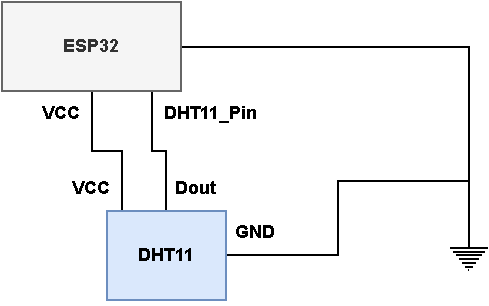
\includegraphics[scale=1]{conexionado_dht11}
    \captionof{figure}{Circuito del conexionado DHT11.}
    \label{fig:conexionado_dht11}
\end{center}




\subsection{Medición de presión}
Para el desarrollo de este prototipo se utilizó el framework ESP-IDF y la biblioteca de código ESP-IDF Components que provee el soporte para gestionar el BMP280. A continuación se puede apreciar el conexionado del prototipo en la figura \ref{fig:conexionado_bmp280} y los detalles de sus pines en la tabla \ref{tab:conexionado_bmp280}.

\vspace{0.5cm}    
\begin{table}[h]
\centering
\caption[Conexionado BMP280]{Conexionado BMP280}
\begin{tabular}{l c }
\toprule
\textbf{Nombre lógico} &  \textbf{Pin GPIO}\\
\midrule
 BMP SDA & 18 \\
 BMP280 SCL & 19  \\
\bottomrule
\hline
\end{tabular}
\label{tab:conexionado_bmp280} 
\end{table}
    
\vspace{0.5cm}    
\begin{center}
  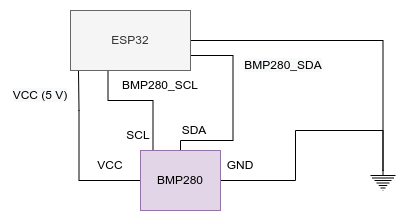
\includegraphics[scale=1]{conexionado_bmp280}
    \captionof{figure}{Conexionado BMP280.}
    \label{fig:conexionado_bmp280}
\end{center}




\subsection{Medición de valor de luminosidad}
Para el desarrollo de este prototipo se utilizó el siguiente conexionado y la biblioteca de código ADC provista por ESP-IDF. A continuación se puede apreciar el conexionado del prototipo en la figura \ref{fig:conexionado_fotoresistor} y los detalles de sus pines en la tabla \ref{tab:conexionado_fotoresistor}.

\vspace{0.5cm}    
\begin{table}[h]
\centering
\caption[Conexionado fotorresistor]{Conexionado fotorresistor}
\begin{tabular}{l c c}
\toprule
\textbf{Nombre lógico} & \textbf{Pin ADC} & \textbf{Pin GPIO}\\
\midrule
ADC Fot pin & channel 0 - unit 2 & 4\\
\bottomrule
\hline
\end{tabular}
\label{tab:conexionado_fotoresistor}
\end{table}


\vspace{0.5cm}
\begin{center}
  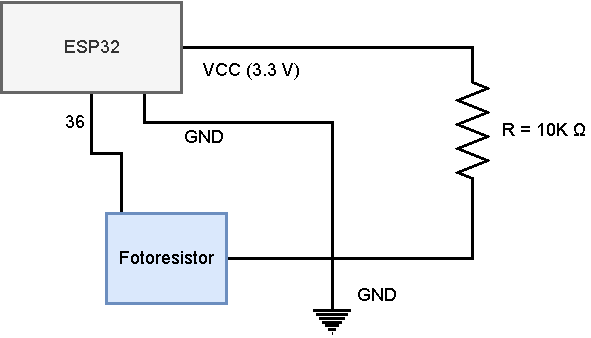
\includegraphics[scale=1]{conexionado_fotoresistor}
    \captionof{figure}{Conexionado fotorresistor.}
    \label{fig:conexionado_fotoresistor}
    
\end{center}
\subsection{Control del joystick analogico}
Para el desarrollo de este prototipo se utilizó el siguiente conexionado y la biblioteca de código ADC provista por ESP-IDF. A continuación se puede apreciar el conexionado del prototipo en la figura \ref{fig:conexionado_joystick} y los detalles de sus pines en la tabla \ref{tab:conexionado_joystick}.


\vspace{0.5cm}
\begin{table}[h]
\centering
\caption[Conexionado joystick]{Conexionado joystick}
\begin{tabular}{l c c}
\toprule
\textbf{Nombre lógico} & \textbf{Pin ADC} & \textbf{Pin GPIO}\\
\midrule
ADC X & channel 1 - unit 2 & 0 \\
ADC Y & channel 7 - unit 1 & 35 \\
\bottomrule
\hline
\end{tabular}
\label{tab:conexionado_joystick}
\end{table}

\vspace{0.5cm}

\begin{center}
  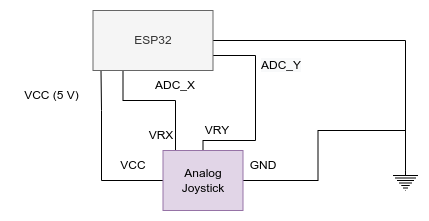
\includegraphics[scale=1]{conexionado_joystick}
    \captionof{figure}{Conexionado joystick.}
    \label{fig:conexionado_joystick}
    

\end{center}

\subsection{Control del display}
 

\subsection{Control de motores DC}


...

\subsection{Control de la red WIFI}


...


\subsection{Gestion de la  de la comunicacion sockets UDP}


...



\section{Arquitectura de hardware del sistema}

Los macro componentes de hardware presentes en la arquitectura son el robot y el joystick.
Internamente se disenio su micro arquitectura de forma modular, de forma tal que se permita la adaptacion de los diferentes componentes de forma independiente.
El conexionado de cada uno de ellos puede apreciase a continuacion:
(conexionado de los modulos)

La integracion de los mismos se realizo mediante el disenio y contruccion de una placa integradora base que permite

\section{Interfaz de usuario}

...



